% Editable v4 design mockup; generated imagery and illustrative motion, not trial evidence.
\begin{center}
\vspace{-6pt}
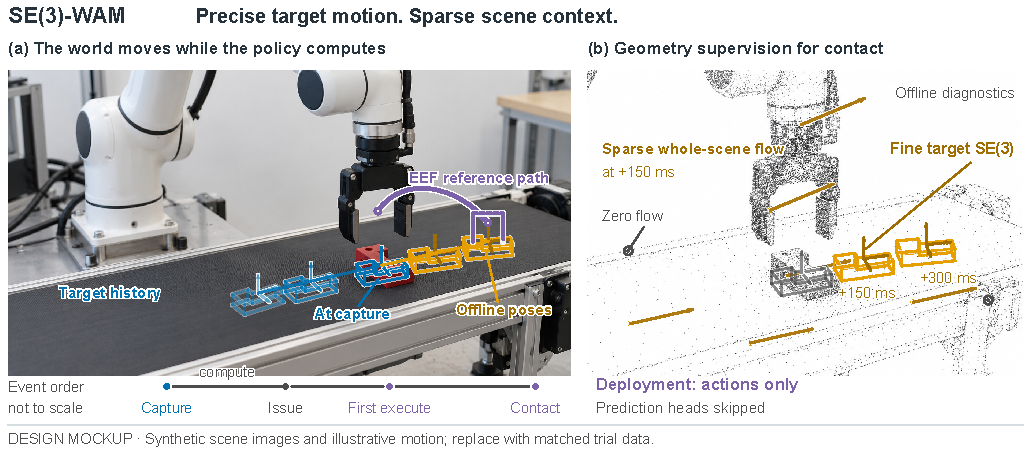
\includegraphics[width=\textwidth]{figures/Fig1/fig1_storyboard.pdf}
\captionof{figure}{\textbf{Learning geometry for dynamic contact.}
(a) Target history (blue), illustrative future poses (orange), and an end-effector reference path (purple) show motion between observation and contact. Capture, issue, first execution, and contact are distinct; the event strip is not to scale.
(b) Fine target SE(3) and sparse whole-scene 3D flow provide training supervision. Horizons are measured from capture; flow is shown at $+150$\,ms, with ringed zero-flow samples on static context. Background points depict scene context, not the supervision grid. Prediction heads are skipped at deployment; decoded geometry does not feed actions.
\emph{Design mockup: both scene images are generated capture-state context; poses, motion, and contact are illustrative, not trial data or model outputs.}}
\label{fig:teaser}
\vspace{4pt}
\end{center}
